\section{Segunda Parte}
\subsection{Implementaci\'on}
\subsubsection{Descripci\'on del problema}
Se pidió en esta segunda parte implementar un parser que parsee texto según la gramática especificada en la sección \ref{sec:gramatica}. Esta implementación debería tomar como entrada una cadena de texto y en caso de poder parsearla, producir como salida un archivo en formato HTML que se pueda abrir desde un browser y que dentro de él, se encuentre el texto procesado de la entrada pero correctamente indentado y coloreado.

Por ejemplo, para la siguiente entrada:

      \begin{verbatim}
<html><head><title>Título</title><script>print("hello")</script>\n
</head><body>\ntexto<p>párrafo<h1><!--comentario--><p> más texto
</p></h1></p>\n <div>texto texto texto <br> mas texto texto texto
</div>\n\n</body>\n</html>\n\end{verbatim}

Se producirá la siguiente salida en un archivo HTML:

\begin{figure}[h!]
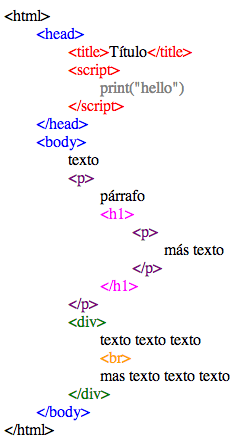
\includegraphics[width=5cm]{img/ejemplo1.png}
      \caption{Salida para un ejemplo válido.}
      \label{tbl:ejemplo}
\end{figure}

\newpage
\subsubsection{Detalles de implementación y limitaciones}
La solución fue desarrollada con ANTLR\footnote{www.antlr.org} y tanto el lexer como el parser generado fueron generados en Java.

El parser no acepta el símbolo \verb|<| dentro de un tag script, podría tokenizarse mejor ya que una comparación dentro del script haría que falle el parsing.

En cuanto a la salida del parsing, esta es calculada en un atributo \textbf{sintetizado} llamado \texttt{texto}. Para manejar la indentación, utilizamos un único tag \verb|<div class="bloque">| cuyo único estilo tiene un margen a izquierda, fijo. El efecto de ir generando estos divs a medida que se necesita generar un tag produce la indentación deseada, contemplando el nivel de encadenamiento de tags producto de ir procesando un tag dentro de otro.

En cuanto al coloreo de los tags, cada tag reconocido tiene su correspondiente código HTML con un estilo (CSS) que le otorga el color.

\subsubsection{Entradas de prueba válidas}

\underline{Entrada 1:}
\begin{verbatim}
<html><head><title>Título</title><script>print("hello")</script>\n
</head><body>\ntexto<p>párrafo<h1><!--comentario--><p> más texto
</p></h1></p>\n <div>texto texto texto <br> mas texto texto texto
</div>\n\n</body>\n</html>\n\end{verbatim}

\underline{Salida 1:}

\begin{figure}[h!]
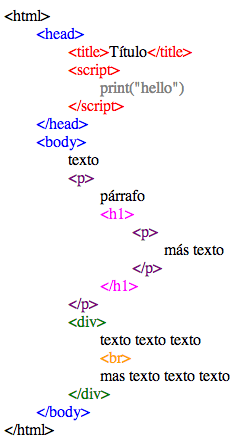
\includegraphics[width=4.8cm]{img/ejemplo1.png}
      \caption{Salida para un ejemplo válido.}
      \label{salida1}
\end{figure}

\underline{Entrada 2:}

\begin{verbatim}
<html>  <head> <script>print("a script")</script><title>Título</title>
 <script>print("hello")</script><script>print("world")</script>\n
</head><body>\ntexto suelto<p>párrafo <h1><!-- comentario--><p> más texto</p></h1>
</p>\n<div>texto texto texto <br> mas texto textotexto</div>\n<div>
Un Div que adentro tiene otro<div>Dentro <div><p>de otro</p> con mas texto
</div></div></div>\n</body>\n</html>\n
\end{verbatim}

\underline{Salida 2:}

\begin{figure}[h!]
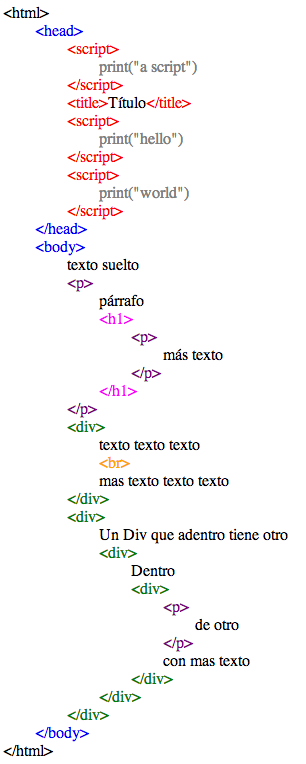
\includegraphics[width=4.8cm]{img/ejemplo2.png}
      \caption{Salida para un ejemplo válido.}
      \label{salida2}
\end{figure}

\newpage 

\subsubsection{Entradas de prueba inválidas}

\underline{Entrada 3 (\texttt{<title>} sin abrir):}
\begin{verbatim}
<html>  Título</title> <script>print("hello")</script><script>print("world")
</script>\n</head><body>\ntexto suelto<p>párrafo <h1><!-- comentario--><p> 
más texto</p></h1></p>\n<div>texto texto texto <br> mas texto texto texto
</div>\n<div>Un Div que adentro tiene otro<div>Dentro <div><p>de otro
</p> con mas texto</div></div></div>\n</body>\n</html>\n
	\end{verbatim}
    
\underline{Salida 3:}
\\\\
\verb|line 1:6 missing TK_C_HTML at ' Título' <html>|\\\\
\underline{Entrada 4 (\texttt{<div>} sin cerrar):}
\\\\
\begin{verbatim}
<html>  <head> <script>print("a script")</script><title>Título</title>
<script>print("hello")</script><script>print("world")</script>\n
</head><body>\ntexto suelto<p>párrafo <h1><!-- comentario--><p> 
más texto</p></h1></p>\n<div>texto texto texto <br> mas texto texto 
texto\n<div>Un Div que adentro tiene otro<div>Dentro <div><p>de otro</p> 
con mas texto</div></div></div>\n</body>\n</html>\n
\end{verbatim}

\underline{Salida 4:}\\\\
{\footnotesize
\verb|line 6:0 mismatched input '<span class="body">&lt;/body&gt;</span>' expecting TK_C_DIV|
}
